\section*{Model descriptions}

\subsection*{Pattern 1}
With this model, we had to find all the activities in the Dreyers log, which we simply did by
making a small Python script. We added an addtional activity called "Case" to avoid having
a condition arrow pointing to each and every one of the activities.
\begin{center}
    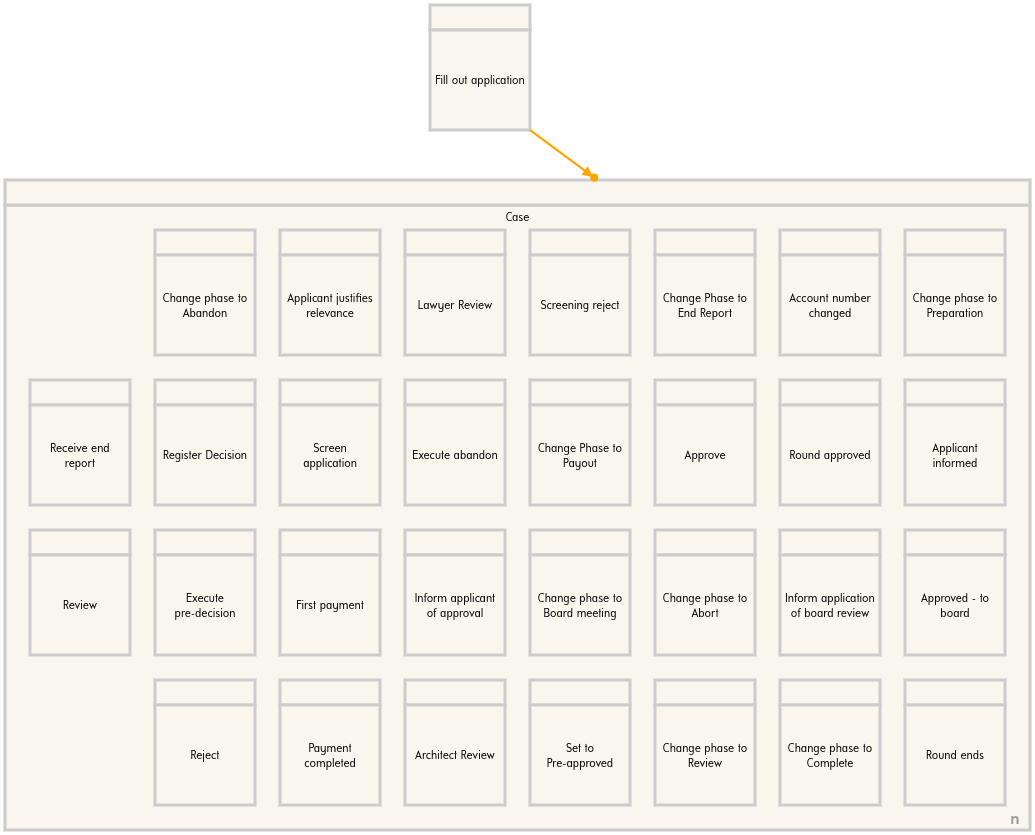
\includegraphics[width=1\textwidth]{pattern_1}
\end{center}	

\newpage
\subsection*{Pattern 2}
Again, we nested the two within an outer activity to only draw one pending arrow.
In the assignment text, however, it is stated that both Applicant informed and Change phase to
Abort should happen after Reject, eventually. We were a bit in doubt whether this should mean that
Applicant informed should happen after Reject and then Change phase to Abort, or if the order is
irrelevant. We chose the latter.
\begin{center}
    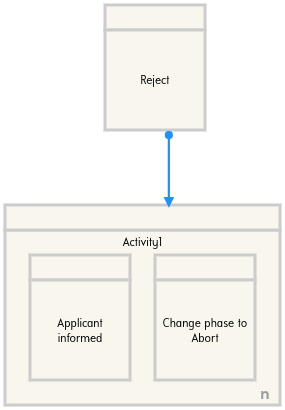
\includegraphics[width=.5\textwidth]{pattern_2}
\end{center}	

\subsection*{Pattern 3}
This simply excludes itself after it has been executed.
\begin{center}
    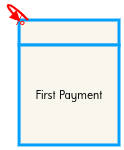
\includegraphics[width=.25\textwidth]{pattern_3}
\end{center}	

\subsection*{Pattern 4}
These simply exclude each other after execution, making sure only one of them is ever executed.
\begin{center}
    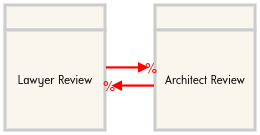
\includegraphics[width=.5\textwidth]{pattern_4}
\end{center}	

